

\tikzset{every picture/.style={line width=0.3pt}} %set default line width to 0.75pt        

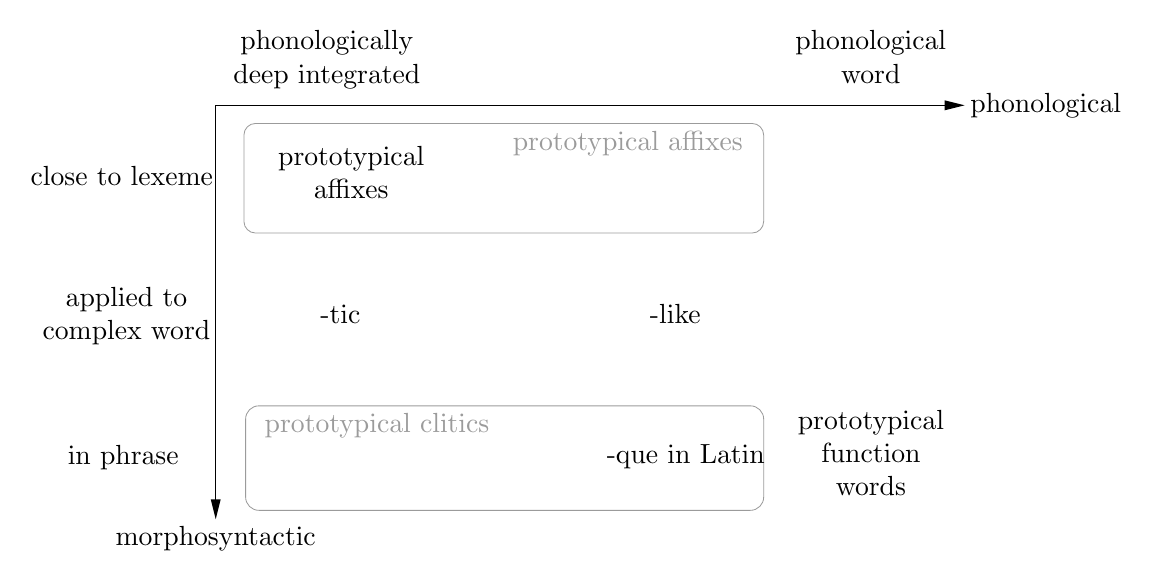
\begin{tikzpicture}[x=0.75pt,y=0.75pt,yscale=-0.8,xscale=0.8]
%uncomment if require: \path (0,370); %set diagram left start at 0, and has height of 370

%Straight Lines [id:da9197142727880097] 
\draw    (166,94) -- (615,94) ;
\draw [shift={(617,94)}, rotate = 180] [fill={rgb, 255:red, 0; green, 0; blue, 0 }  ][line width=0.08]  [draw opacity=0] (12,-3) -- (0,0) -- (12,3) -- cycle    ;
%Straight Lines [id:da7092949523578058] 
\draw    (166,94) -- (166,341.26) ;
\draw [shift={(166,343.26)}, rotate = 270] [fill={rgb, 255:red, 0; green, 0; blue, 0 }  ][line width=0.08]  [draw opacity=0] (12,-3) -- (0,0) -- (12,3) -- cycle    ;
%Rounded Rect [id:dp687660284833467] 
\draw  [color={rgb, 255:red, 155; green, 155; blue, 155 }  ,draw opacity=1 ] (184,283) .. controls (184,278.58) and (187.58,275) .. (192,275) -- (488,275) .. controls (492.42,275) and (496,278.58) .. (496,283) -- (496,329.93) .. controls (496,334.35) and (492.42,337.93) .. (488,337.93) -- (192,337.93) .. controls (187.58,337.93) and (184,334.35) .. (184,329.93) -- cycle ;
%Rounded Rect [id:dp1009576986560572] 
\draw  [color={rgb, 255:red, 155; green, 155; blue, 155 }  ,draw opacity=1 ] (183,111.93) .. controls (183,108.06) and (186.13,104.93) .. (190,104.93) -- (489,104.93) .. controls (492.87,104.93) and (496,108.06) .. (496,111.93) -- (496,163.93) .. controls (496,167.79) and (492.87,170.93) .. (489,170.93) -- (190,170.93) .. controls (186.13,170.93) and (183,167.79) .. (183,163.93) -- cycle ;

% Text Node
\draw (619,94) node [anchor=west] [inner sep=0.75pt]   [align=left] {phonological};
% Text Node
\draw (166,346.26) node [anchor=north] [inner sep=0.75pt]   [align=left] {morphosyntactic};
% Text Node
\draw (53,129) node [anchor=north west][inner sep=0.75pt]   [align=left] {close to lexeme};
% Text Node
\draw (57,202) node [anchor=north west][inner sep=0.75pt]   [align=left] {\begin{minipage}[lt]{64.47pt}\setlength\topsep{0pt}
\begin{center}
applied to \\complex word
\end{center}

\end{minipage}};
% Text Node
\draw (72.5,297) node [anchor=north west][inner sep=0.75pt]   [align=left] {\begin{minipage}[lt]{43.56pt}\setlength\topsep{0pt}
\begin{center}
in phrase
\end{center}

\end{minipage}};
% Text Node
\draw (169,47.5) node [anchor=north west][inner sep=0.75pt]   [align=left] {\begin{minipage}[lt]{74.92pt}\setlength\topsep{0pt}
\begin{center}
phonologically\\ deep integrated
\end{center}

\end{minipage}};
% Text Node
\draw (510.5,47.5) node [anchor=north west][inner sep=0.75pt]   [align=left] {\begin{minipage}[lt]{58.21pt}\setlength\topsep{0pt}
\begin{center}
phonological\\word
\end{center}

\end{minipage}};
% Text Node
\draw (199,117) node [anchor=north west][inner sep=0.75pt]   [align=left] {\begin{minipage}[lt]{56.52pt}\setlength\topsep{0pt}
\begin{center}
prototypical\\affixes
\end{center}

\end{minipage}};
% Text Node
\draw (400,297) node [anchor=north west][inner sep=0.75pt]   [align=left] {\mbox{-}que in Latin};
% Text Node
\draw (512,276) node [anchor=north west][inner sep=0.75pt]   [align=left] {\begin{minipage}[lt]{56.52pt}\setlength\topsep{0pt}
\begin{center}
prototypical\\function\\words
\end{center}

\end{minipage}};
% Text Node
\draw (426,212.5) node [anchor=north west][inner sep=0.75pt]   [align=left] {\mbox{-}like};
% Text Node
\draw (227.5,212.5) node [anchor=north west][inner sep=0.75pt]   [align=left] {\mbox{-}tic};
% Text Node
\draw (194,278) node [anchor=north west][inner sep=0.75pt]  [color={rgb, 255:red, 155; green, 155; blue, 155 }  ,opacity=1 ] [align=left] {prototypical clitics};
% Text Node
\draw (485,107.93) node [anchor=north east] [inner sep=0.75pt]  [color={rgb, 255:red, 155; green, 155; blue, 155 }  ,opacity=1 ] [align=left] {prototypical affixes};


\end{tikzpicture}
